\documentclass[UTF8]{ctexart}
\usepackage{../Zhihu}
\title{数字电路学习笔记(十一):时序逻辑}
\begin{document}
\maketitle
\textit{时序逻辑将会是本笔记的最后几章的主题。虽然数字电路课程还包括脉冲电路、模数转换、EDA等内容,但那些和本文的主线内容(不注重硬件搭建的电路设计)关系就不大了。}

\section*{一、时序功能}
我们从一个例子开始,说明时序逻辑的概念和作用。

\begin{quote}
设计一个电路,当连续输入四个及以上的高电平时,输出高电平;其他时候,输出低电平。
这个需求显然无法用我们已设计过的任何组合逻辑电路实现:因为对于组合逻辑,每一次工作都是独立的,“连续输入四个高电平”这样的场景无法出现(但是,我们可以做出一个检验“同时输入四个高电平”的电路;品味这其中的区别)。因此,我们需要借助时序电路的时序功能。
\end{quote}

时序电路和组合逻辑电路类似,我们最为关心的是它的输入(命名为$X$)和输出(命名为$Y$),在此题中,已经有了良定义的输入输出;同时,时序逻辑电路还会拥有一组自身的状态。比如对于上述的需求,可以用两位来存储输入的高电平的数量:$Q_1Q_0$。当$Q_1Q_0=11$时,每次输入一个高电平,即认为已经“连续输入了四个以上的高电平”,输出高电平;其他时候,则根据输入决定是状态+1还是状态归0。这样的文字表述,我们可以用这样一张状态转换图做可视化:

\begin{figure}
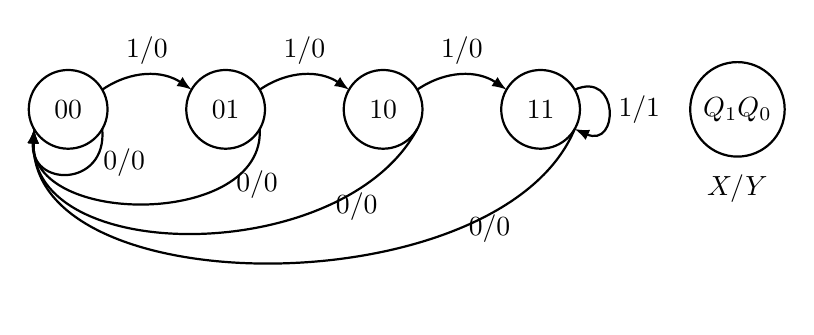
\begin{tikzpicture}[scale=1]
    \draw[thick] (0,2) node {$00$} circle[radius=0.5];
    \draw[thick] (2,2) node {$01$} circle[radius=0.5];
    \draw[thick] (4,2) node {$10$} circle[radius=0.5];
    \draw[thick] (6,2) node {$11$} circle[radius=0.5];
    \foreach \x in {0,2,4}
    \draw[thick,-latex] ([shift={(30:0.5)}]\x,2) .. controls ({\x+0.8},2.5) and ({\x+1.2},2.5) .. node[above] {1/0} ([shift={(150:0.5)}]{\x+2},2);
    \draw[thick,-latex] ([shift={(-30:0.5)}]0,2) .. controls (0.5,1) and (-0.5,1) .. node[near start, right] {0/0} ([shift={(210:0.5)}]0,2);
    \draw[thick,-latex] ([shift={(-30:0.5)}]2,2) .. controls (2.5,0.5) and (-0.5,0.5) .. node[near start, right] {0/0} ([shift={(210:0.5)}]0,2);
    \draw[thick,-latex] ([shift={(-30:0.5)}]4,2) .. controls (3.5,0) and (-0.5,0) .. node[near start, right] {0/0} ([shift={(210:0.5)}]0,2);
    \draw[thick,-latex] ([shift={(-30:0.5)}]6,2) .. controls (5.5,-0.5) and (-0.5,-0.5) .. node[near start, right] {0/0} ([shift={(210:0.5)}]0,2);
    \draw[thick,-latex] ([shift={(30:0.5)}]6,2) .. controls (7,2.5) and (7,1.5) .. node[right] {1/1} ([shift={(-30:0.5)}]6,2);
    \draw[thick] (8.5,2) node {$Q_1Q_0$} circle[radius=0.6];
    \node at (8.5,1) {$X/Y$};
\end{tikzpicture}
\end{figure}

在前两章中,已经出现了一些简单的状态转换图。为了理解这张图,我们首先确定电路的初始状态——在此图中,是最左边的00的圈;接着,顺着箭头,看状态是如何变化的。每个箭头上都写着状态转换所对应的输入输出——至于具体的对应,要看右边的图例,比如此处就标明,斜杠左边为输入$X$,右边为输出$Y$。如果我们在状态为00时输入1,则跳转到01状态;否则保持00状态。接下来每次输入1,则跳转到下一个状态;输入0,则跳转回00。但对于以上所有状态转换,输出都是0。直到状态变成11时,才会在输入1时输出1。

观察状态转换图,发现每个状态的“指入箭头”数目不定,但“指出箭头”数目在输出位数为$n$时一定是$2^n$(可以重合)。否则,就会有“未定义的状态转移”。

对于时序逻辑电路的分析,和对有限状态机 (Finite state machine) 是一样的。事实上,可以把时序逻辑电路看作有限状态机的一种实现形式,许多有限状态机的概念也可以运用到电路中来。可以以下面这篇文章为参考。

\href{https://zhuanlan.zhihu.com/p/28142401}{陈天:谈谈状态机}

\section*{二、时序逻辑电路的信息流}
对一个电路的整体功能有了理解之后,我们可以进一步研究在这个系统中的信息流动。(注意,在这一部分,我们并不关注电路的实际实现,而是从更高、更抽象的观点研究它。)

时序逻辑电路可以分为两部分:存储电路和组合逻辑电路。组合逻辑和时序逻辑与其说是“平行关系”,不如说是“继承关系”。如果组合逻辑电路可以用下图表示(见笔记(六):组合逻辑电路):

\begin{figure}
\begin{tikzpicture}
    \tikzset{style={align=center}};
    \draw[thick] (0,0) rectangle node {组合逻\\辑电路} (1.5,2); 
    \draw[thick,-latex] (-1,1.7) node[left] {$x_1$} -- (0,1.7);
    \draw[thick,-latex] (-1,1.2) node[left] {$x_2$} -- (0,1.2);
    \draw[thick,-latex] (-1,0.3) node[left] {$x_n$} -- (0,0.3);
    \node[rotate=90] at (-0.5,0.75) {...};
    \draw[thick,-latex] (1.5,1.7) -- (2.5,1.7) node[right] {$y_1$};
    \draw[thick,-latex] (1.5,1.2) -- (2.5,1.2) node[right] {$y_2$};
    \draw[thick,-latex] (1.5,0.3) -- (2.5,0.3) node[right] {$y_n$};
    \node[rotate=90] at (2,0.75) {...};
\end{tikzpicture}
\end{figure}

那么时序逻辑电路不过是再加一个辅助的存储电路:

\begin{figure}
\begin{tikzpicture}
    \tikzset{style={align=center}};
    \draw[thick] (0,-0.5) rectangle node {组合逻\\辑电路} (2,2); 
    \draw[thick,-latex] (-1,1.7) node[left] {$x_1$} -- ++(1,0);
    \draw[thick,-latex] (-1,1.3) node[left] {$x_2$} -- ++(1,0);
    \draw[thick,-latex] (-1,0.7) node[left] {$x_n$} -- ++(1,0);
    \node[rotate=90] at (-0.5,1) {...};
    \draw[thick,-latex] (2,1.7) -- ++(1,0) node[right] {$y_1$};
    \draw[thick,-latex] (2,1.3) -- ++(1,0) node[right] {$y_2$};
    \draw[thick,-latex] (2,0.7) -- ++(1,0) node[right] {$y_n$};
    \node[rotate=90] at (2.5,1) {...};
    \draw[thick] (0,-2.5) rectangle node {存储电路} (2,-1);
    \draw[thick,-latex] (2,0.3) -- (3,0.3) -- (3,-2.2) -- (2,-2.2) node[below right] {$z_n$};
    \draw[thick,-latex] (2,-0.1) -- (2.6,-0.1) -- (2.6,-1.3) -- (2,-1.3) node[above right] {$z_1$};
    \draw[thick,-latex] (0,-2.2) node[below left] {$q_n$} -- (-1,-2.2) -- (-1,0.3) -- (0,0.3);
    \draw[thick,-latex] (0,-1.3) node[above left] {$q_1$} -- (-0.6,-1.3) -- (-0.6,-0.1) -- (0,-0.1);
    \node[rotate=90] at (-0.3,-1.75) {...};
    \node[rotate=90] at (2.3,-1.75) {...};
\end{tikzpicture}
\end{figure}

其中$x_1,x_2,\dots,x_n$以及$y_1,y_2,\dots,y_n$是我们熟悉的输入$X$和输出$Y$。事实上,应该是向量形式的$\mathbf{X}$和$\mathbf{Y}$,但没有必要做这种区分,造成更多的困惑。

实际输入存储电路的并不是输入本身,而是已经经过处理的内部输入信号$Z$。它控制了由锁存器和触发器组成的存储电路。存储电路又会产生内部输出信号$Q$,也就是它的状态。

回忆组合逻辑电路的方程,我们给出了一般形式$Y=F(X)$,表示输出完全由输入决定。对于时序逻辑,我们发现有两组“自变量”,也就是外部输入$X$与电路状态$Q$。我们定义如下三组方程(我花了点时间试着通过例子来合理化这些方程,但最后发现还是直接把它们作为定义更合理。在后续的实际电路设计中,能对它们的意义有更好地理解):

\begin{equation*}
    \begin{aligned}
        输出方程:Y&=F(X,Q)\\
        驱动方程:Z&=G(X,Q)\\
        状态方程:Q^*&=H(X,Q)\\
    \end{aligned}
\end{equation*}

这些方程可以通过上图得出。

注意,状态并不是实时更新的——不然可以想见,由于有$Q^*=H(X,Q)$,对于任何一个输入,状态一定会落到一个$Q\equiv H(X,Q)$的稳态上,但这种稳态的数量是非常有限的。事实上,时序逻辑电路的存储电路仍由时钟信号控制,只有在一个时钟信号的边沿发生单次状态更新。

还有两个概念可以在这里提出:

\begin{itemize}
\item 由于存储电路由不止一个触发器构成,每个触发器都需要一个时钟信号,这些时钟信号可以由同一个信号源给出,同时更新,也可以分别更新。前者称为同步电路,后者称为异步电路。下文中所有电路都为同步电路。
\item 有些电路没有外部输入信号,而完全依靠时钟信号进行状态更新;另一些的输入信号只影响状态,而不决定输出。对于两种情况,输出都只与状态有关($Y=F(Q)$)。这种电路称为Moore型电路。而$Y=F(X,Q)$的则称为Mealy型电路。
\end{itemize}

这一节非常抽象,提出了很多定义和公式。事实上,第一遍学习时不完全理解问题不大,但通过后续逐步介绍的电路设计,可以对时序逻辑有更深刻的认识。

\section*{三、时序电路的功能表示}
\subsection*{1、状态转换表}
在组合逻辑中,我们用真值表对功能做了最具象的表达。对于时序逻辑,虽然需要同时研究输入、输出和状态的相互作用关系,但真值表也可以达到同样的效果。在时序逻辑中,真值表叫做状态转换表。

\begin{figure}
    \begin{tabular}{|c|c|c|c|c|}\hline\rowcolor{lightgray}
        &\multicolumn{2}{c|}{$Q^*_1Q^*_0$}&\multicolumn{2}{c|}{$Y$}\\\cline{2-5}\rowcolor{lightgray}
        \multirow{-2}{*}{$Q_1Q_0$}&$X=0$&$X=1$&$X=0$&$X=1$\\\hline
        00&00&01&0&0\\\hline
        01&00&10&0&0\\\hline
        10&00&11&0&0\\\hline
        11&00&11&0&1\\\hline
    \end{tabular}
\end{figure}

通过该真值表,我们可以用一样的思路列出各个方程。

上图可能和一般的真值表有稍许不同——因为我们把$X$的值横向排列而不是像一般的做法一样纵向排列,这样可以缩短表格长度,也更加强调“状态转换”的关系。但是画成下图这样也是一样的:

\begin{figure}
    \begin{tabular}{|c|c|c|c|}\hline\rowcolor{lightgray}
        $X$&$Q_1Q_0$&$Q^*_1Q^*_0$&$Y$\\\hline
        0&00&00&0\\\hline
        0&01&00&0\\\hline
        0&10&00&0\\\hline
        0&11&00&0\\\hline
        1&00&01&0\\\hline
        1&01&10&0\\\hline
        1&10&11&0\\\hline
        1&11&11&1\\\hline
    \end{tabular}
\end{figure}

\subsection*{2、状态转换图}
在时序逻辑设计中,状态转换图是比转换表更加直观的表示方法。就像之前给出的示例一样:

\begin{figure}
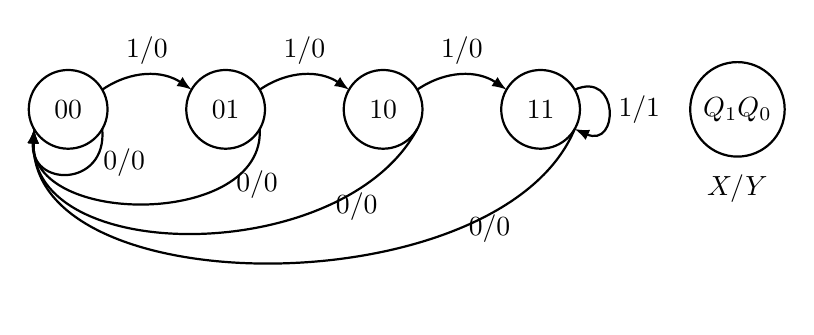
\begin{tikzpicture}[scale=1]
    \draw[thick] (0,2) node {$00$} circle[radius=0.5];
    \draw[thick] (2,2) node {$01$} circle[radius=0.5];
    \draw[thick] (4,2) node {$10$} circle[radius=0.5];
    \draw[thick] (6,2) node {$11$} circle[radius=0.5];
    \foreach \x in {0,2,4}
    \draw[thick,-latex] ([shift={(30:0.5)}]\x,2) .. controls ({\x+0.8},2.5) and ({\x+1.2},2.5) .. node[above] {1/0} ([shift={(150:0.5)}]{\x+2},2);
    \draw[thick,-latex] ([shift={(-30:0.5)}]0,2) .. controls (0.5,1) and (-0.5,1) .. node[near start, right] {0/0} ([shift={(210:0.5)}]0,2);
    \draw[thick,-latex] ([shift={(-30:0.5)}]2,2) .. controls (2.5,0.5) and (-0.5,0.5) .. node[near start, right] {0/0} ([shift={(210:0.5)}]0,2);
    \draw[thick,-latex] ([shift={(-30:0.5)}]4,2) .. controls (3.5,0) and (-0.5,0) .. node[near start, right] {0/0} ([shift={(210:0.5)}]0,2);
    \draw[thick,-latex] ([shift={(-30:0.5)}]6,2) .. controls (5.5,-0.5) and (-0.5,-0.5) .. node[near start, right] {0/0} ([shift={(210:0.5)}]0,2);
    \draw[thick,-latex] ([shift={(30:0.5)}]6,2) .. controls (7,2.5) and (7,1.5) .. node[right] {1/1} ([shift={(-30:0.5)}]6,2);
    \draw[thick] (8.5,2) node {$Q_1Q_0$} circle[radius=0.6];
    \node at (8.5,1) {$X/Y$};
\end{tikzpicture}
\end{figure}

从一张图上,就可以读出许多输入/输出/状态的对应关系,对于它们之间的影响关系也要比转换表直观。因此,它一般是逻辑设计的第一步,而后再根据该图填写转换表或卡诺图,列方程。

\subsection*{3、卡诺图}
令我绘制得非常痛苦的一类图表。也可以表示输出和次态是如何受输入和现态影响的。由于在时序逻辑中有较多的无关项(具体例子会在后文给出),卡诺图可以极大地方便列方程的过程。

\begin{figure}
    \begin{tabular}{rc|c|c|c|}
        \multirow{2}{*}{\backslashbox{$X$}{$Q_1Q_0$}}&\multicolumn{1}{r}{}&\multicolumn{1}{r}{}&\multicolumn{1}{r}{}&\multicolumn{1}{r}{}\\
        &\multicolumn{1}{r}{\makebox[2em]{00}}&\multicolumn{1}{r}{\makebox[2em]{01}}&\multicolumn{1}{r}{\makebox[2em]{11}}&\multicolumn{1}{r}{\makebox[2em]{10}}\\\cline{2-5}
        \multicolumn{1}{r|}{0}&00/0&00/0&00/0&00/0\\\cline{2-5}
        \multicolumn{1}{r|}{1}&01/0&10/0&11/1&11/0\\\cline{2-5}
    \end{tabular}
\end{figure}

\subsection*{4、状态方程}
也就是之前列出的三组方程:

\begin{equation*}
    \begin{aligned}
        输出方程:Y&=F(X,Q)\\
        驱动方程:Z&=G(X,Q)\\
        状态方程:Q^*&=H(X,Q)\\
    \end{aligned}
\end{equation*}

当我们成功列出方程后,离设计实际电路就只有一步之遥了。

以上便是几种常用的时序逻辑电路功能表示方法。它们都是在绘制电路前不可缺少的步骤,也是理解电路功能必需的工具。

\divider

本章非常抽象,我也花了很大功夫试图合理化抛出的每个概念。但4个月后,我仍然对我的成果不满意。希望各位可以提出你们的意见,并感谢各位在我断更的四个月内对我的支持:)

% \begin{figure}
% \begin{tikzpicture}[scale=1]
%     \draw[thick] (0,2) node {$000$} circle[radius=0.5];
%     \draw[thick] (2,2) node {$001$} circle[radius=0.5];
%     \draw[thick] (4,2) node {$010$} circle[radius=0.5];
%     \draw[thick] (6,2) node {$011$} circle[radius=0.5];
%     \draw[thick] (6,0) node {$100$} circle[radius=0.5];
%     \draw[thick] (4,0) node {$101$} circle[radius=0.5];
%     \draw[thick] (2,0) node {$110$} circle[radius=0.5];
%     \draw[thick] (0,0) node {$111$} circle[radius=0.5];
%     \foreach \x in {0,2,4}
%     \draw[thick,-latex] ([shift={(30:0.5)}]\x,2) .. controls ({\x+0.8},2.5) and ({\x+1.2},2.5) .. node[above] {/0} ([shift={(150:0.5)}]{\x+2},2);
%     \foreach \x in {0,2,4}
%     \draw[thick,-latex] ([shift={(210:0.5)}]{\x+2},0) .. controls ({\x+1.2},-0.5) and ({\x+0.8},-0.5) .. node[below] {/0} ([shift={(-30:0.5)}]\x,0);
%     \draw[thick,-latex] ([shift={(-60:0.5)}]6,2) .. controls (6.5,1.2) and (6.5,0.8) .. node[right] {/0} ([shift={(60:0.5)}]6,0);
%     \draw[thick,-latex] ([shift={(120:0.5)}]0,0) .. controls (-0.5,0.8) and (-0.5,1.2) .. node[left] {/1} ([shift={(-120:0.5)}]0,2);
%     \draw[thick] (8,1) node {$Q_2Q_1Q_0$} circle[radius=0.7];
%     \node at (8,0) {$/Y$};
% \end{tikzpicture}
% \end{figure}
\end{document}
